\documentclass[12pt,letterpaper]{article}     	

% Paquetes de generalidades
%%%%%%%%%%%%%%%%%%%%%%%%%%%%%%%

% Para escribir tildes y eñes
\usepackage{multirow}
\usepackage[utf8]{inputenc}
\usepackage[T1]{fontenc}
\usepackage{mathtools}
\usepackage{subcaption}
\usepackage{listings}
\usepackage[makeroom]{cancel}
\usepackage{graphicx}
\usepackage{xcolor}
\usepackage{csquotes}
\expandafter\def\csname ver@subfig.sty\endcsname{}
\newcommand\mybar{\kern1pt\rule[-\dp\strutbox]{.8pt}{\baselineskip \space}\kern1pt}




% Para que los títulos de figuras, tablas y otros estén en español
\usepackage[spanish,es-noquoting]{babel} 
	% Cambiar nombre a tablas
	\addto\captionsspanish{\renewcommand{\tablename}{Tabla}}	
    % Cambiar nombre a lista de tablas		
	\addto\captionsspanish{\renewcommand{\listtablename}{Índice de tablas}}	
    % Cambiar nombre a capítulos
	\addto\captionsspanish{\renewcommand{\chaptername}{Sección}}

% Para que la bibligrafía esté en español
\usepackage[fixlanguage]{babelbib}
\selectbiblanguage{spanish}

% Tamaño del área de escritura de la página	
\usepackage{geometry}                         
	\geometry{left=18mm,right=18mm,top=23mm,bottom=23mm} 	

% Paquetes para matemática
%%%%%%%%%%%%%%%%%%%%%%%%%%%%%%%

% Los paquetes ams son desarrollados por la American Mathematical Society y mejoran la escritura de fórmulas y símbolos matemáticos.
\usepackage{amsmath}       
\usepackage{amsfonts}     	
\usepackage{amssymb}

% Paquetes para manejo de gráficas y figuras
%%%%%%%%%%%%%%%%%%%%%%%%%%%%%%%

% Para insertar gráficas
\usepackage{graphicx}     	


% Para crear gráficos vectoriales con un lenguaje descriptivo/geométrico
\usepackage{tikz}

% Para crear circuitos vectoriales basados en TikZ
\usepackage[american]{circuitikz}

% Paquetes relacionados con el estilo 
%%%%%%%%%%%%%%%%%%%%%%%%%%%%%%%

% Para la presentación correcta de magnitudes y unidades
\usepackage{siunitx}	

% Para incluir documentos pdf
\usepackage{pdfpages}
\usepackage{animate}
% Para hipervínculos y marcadores
\usepackage[colorlinks=true,urlcolor=black,linkcolor=black,citecolor=black]{hyperref}
	\urlstyle{same}

% Para ubicar las tablas y figuras justo después del texto
\usepackage{float}	
\usepackage{enumitem}
% Para hacer tablas más estilizadas
\usepackage{booktabs}		

% Para hacer secciones con múltiples columnas
\usepackage{multicol}

% Para insertar código fuente estilizado


% Para agregar código con formato de Matlab
\usepackage[numbered,autolinebreaks]{mcode}

% Para utilizar el número de páginas
\usepackage{lastpage}

% Para manejar los encabezados y pies de página
\usepackage{fancyhdr}
	% Contenido de los encabezados y pies de pagina
	\pagestyle{fancy}

% Misceláneos
%%%%%%%%%%%%%%%%%%%%%%%%%%%%%%%

% Para insertar símbolos extraños
\usepackage{marvosym}
%\renewcommand{\theenumi}{\alph{enumi}}

	\lhead{IE-0624 Laboratorio de Microcontroladores}
	\chead{}
	\rhead{}
	\lfoot{Escuela de Ingeniería Eléctrica}
	\cfoot{\thepage\ de \pageref{LastPage}}
	\rfoot{Universidad de Costa Rica}

\newcommand{\EIE}{\textsc{Escuela \Lightning~ Ingeniería Eléctrica}}

\begin{document}


\author{Dylan Agüero Carrillo B90083 \\
        Noel Blandón Saborío  B61097 \\
        [10mm] {Grupo 01}\\ [10mm] Profesor: MSc. Marco Villalta Fallas\\ [20mm]}

\title{%
{\large{\sc Universidad de Costa Rica}} \\[-2mm] {\large Escuela de Ingeniería Eléctrica} \\[-2mm] {\large IE-0624 Laboratorio de Microcontroladores} \\[20mm]
% Título aquí:
Laboratorio 2: GPIOs, Timers y FSM\\ [20mm]
}

\date{14 de abril de 2024}

\pdfbookmark[1]{Portada}{portada} 	% Marcador para el título
\maketitle							% Título
\thispagestyle{empty}

\newpage
\pagenumbering{arabic} 
\setlength{\parindent}{0.6cm}
\setlength{\parskip}{0.25cm}

\section{Introducción}
En el presente reporte de laboratorio se exponen los resultados obtenidos empleando el microcontrolador ATtiny4313. Con esto se plantea el desarrollo de una serie de semáforos, esto empleando los conceptos relacionados a los pines de entrada y salida, los timers propios del microcontrolador y la aplicación de máquinas de estado para poder desarrollar el código correspondiente.


\section{Nota teórica}
\subsection{Especificaciones del ATtiny4313}
El ATtiny4313 es un microcontrolador AVR de 8 bits de alto rendimiento y bajo consumo de energía. Presenta dos temporizadores/contadores, interrupciones externas e internas. Además, debido a sus características internas lo convierte en un microcontrolador potente, el cual puede ejecutar instrucciones incluso en un solo ciclo de reloj. Con esto en cuenta se tienen las siguientes características del dispositivo\cite{Microchip_Technology_2011}:


\begin{table}[H]
\centering
\caption{Características del ATtiny4313}
\label{001}
\begin{tabular}{|c|c|}
\hline
{\color[HTML]{222222} }                                                            & {\color[HTML]{000000} }                                       \\
\multirow{-2}{*}{{\color[HTML]{222222} \textbf{Procesador de núcleo}}}             & \multirow{-2}{*}{{\color[HTML]{000000} AVR}}                  \\ \hline
{\color[HTML]{222222} }                                                            & {\color[HTML]{444444} }                                       \\
\multirow{-2}{*}{{\color[HTML]{222222} \textbf{Tamaño de núcleo}}}                 & \multirow{-2}{*}{{\color[HTML]{444444} 8 bits}}               \\ \hline
{\color[HTML]{222222} }                                                            & {\color[HTML]{444444} }                                       \\
\multirow{-2}{*}{{\color[HTML]{222222} \textbf{Velocidad}}}                        & \multirow{-2}{*}{{\color[HTML]{444444} 20MHz}}                \\ \hline
{\color[HTML]{222222} }                                                            & {\color[HTML]{444444} }                                       \\
\multirow{-2}{*}{{\color[HTML]{222222} \textbf{Conectividad}}}                     & \multirow{-2}{*}{{\color[HTML]{444444} I2C, SPI, UART/USART}} \\ \hline
{\color[HTML]{222222} }                                                            & {\color[HTML]{444444} }                                       \\
\multirow{-2}{*}{{\color[HTML]{222222} \textbf{N.° de entradas/salidas}}}          & \multirow{-2}{*}{{\color[HTML]{444444} 18}}                   \\ \hline
{\color[HTML]{222222} }                                                            & {\color[HTML]{444444} }                                       \\
\multirow{-2}{*}{{\color[HTML]{222222} \textbf{Capacidad de memoria de programa}}} & \multirow{-2}{*}{{\color[HTML]{444444} 4KB (2K x 16)}}        \\ \hline
                                                                                   &                                                               \\
\multirow{-2}{*}{\textbf{Tipo de memoria de programa}}                             & \multirow{-2}{*}{Memoria flash}                               \\ \hline
                                                                                   &                                                               \\
\multirow{-2}{*}{\textbf{Tamaño de EEPROM}}                                        & \multirow{-2}{*}{256 x 8}                                     \\ \hline
                                                                                   &                                                               \\
\multirow{-2}{*}{\textbf{Capacidad de RAM}}                                        & \multirow{-2}{*}{256 x 8}                                     \\ \hline
                                                                                   &                                                               \\
\multirow{-2}{*}{\textbf{Voltaje - Suministro (Vcc/Vdd)}}                          & \multirow{-2}{*}{1.8V $\sim$5.5V}                             \\ \hline
                                                                                   &                                                               \\
\multirow{-2}{*}{\textbf{Tipo de oscilador}}                                       & \multirow{-2}{*}{Interno}                                     \\ \hline
\end{tabular}
\end{table}


\newpage


Se puede observar el siguiente diagrama correspondiente al microcontrolador\cite{Microchip_Technology_2011}:

\begin{figure}[H]
    \centering
    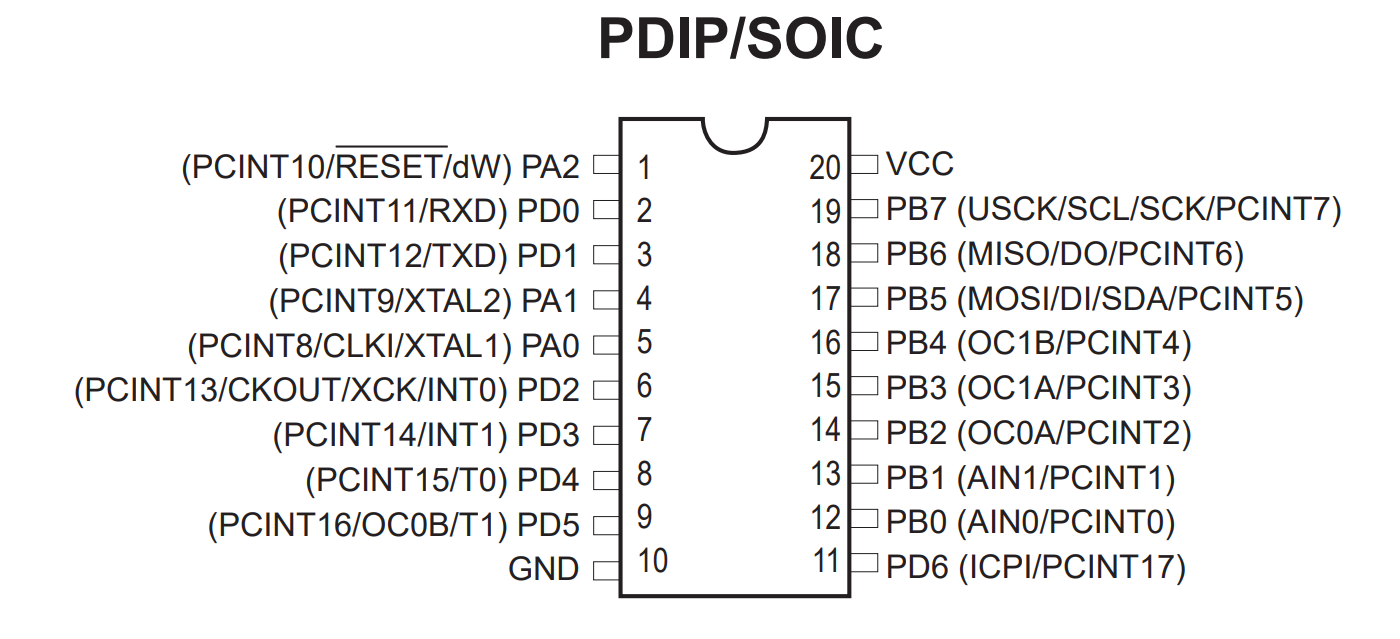
\includegraphics[width=15cm]{Imagenes/diagrama4313.png}
    \caption{Diagrama del microcontrolador ATtiny4313}
    \label{Diagrama del microcontrolador ATtiny4313}
\end{figure}

Por otra parte, se tiene el diagrama de bloques correspondiente al microcontrolador empleado:

\begin{figure}[H]
    \centering
    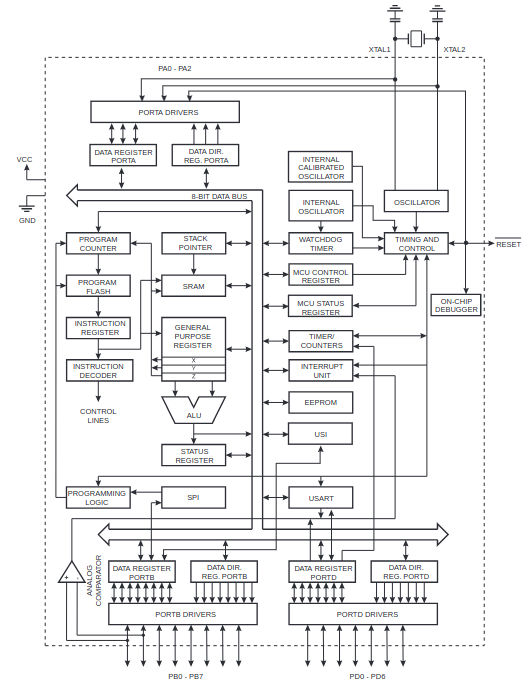
\includegraphics[width=9cm]{Imagenes/block.png}
    \caption{Diagrama de bloques del microcontrolador ATtiny4313}
    \label{Diagrama de bloques del microcontrolador ATtiny4313}
\end{figure}

\newpage

\subsection{Diseño componentes del circuito}
Para los LEDs que indican el comportamiento de los semáforos, se tienen que proteger mediante resistores. Para ello se toman las caraterísticas de los LEDs, en donde la corriente máxima y la tensión eléctrica corresponde son dos valores importantes para el correcto funcionamiento. 
\begin{table}[H]
\centering
\caption{Valores de los LEDs}
\label{tab2}
\begin{tabular}{|l|l|}
\hline
Tensión de alimentación & 5V   \\ \hline
Corriente máxima        & 40mA \\ \hline
Tensión del LED         & 2V   \\ \hline
\end{tabular}
\end{table}

Con esto en cuenta, se calcula el valor correspondiente para los resistores, esto aplicando Ley de Ohm:

\begin{equation}
    R=\frac{5V-2V}{30mA} = 100\Omega
\end{equation}

Se establece la corriente en \textit{30mA} para dejar un margen suficiente antes del valor de la corriente máxima.\\ 

Por otra parte, al requerir el uso de botones, estos provocan la presencia de rebotes indeseados a la hora de ejecutar el programa, es por ello que se emplea un circuito RC que permita eliminar los rebotes\cite{Christoffersen_2015}.\\
Se tiene la siguiente relación:

\begin{equation}
    \tau = RC
\end{equation}

Si se desea un tiempo de aproximadamente 0.1 segundos, se tiene que fijar al menos una de las variables, en este caso se define el resistor en \textit{$1k\Omega$}. Con esto se puede calcular el valor del capacitor:

\[ 0.1s = 1k\Omega\cdot C\]

\begin{equation}
    C = \frac{0.1s}{1k\Omega} = 100\mu C
\end{equation}

Por lo tanto, se tienen los valores requeridos para evitar el rebote al momento de acciones los botones para solicitar el cambio de comportamiento en los semáforos.


\section{Desarrollo/Análisis de resultados}
\subsection{Análisis electrónico}


\subsection{Análisis del programa}



\subsection{Muestra del funcionamiento}


\newpage
\section{Conclusiones y recomendaciones}


\bibliographystyle{IEEEtran}
\bibliography{biblio}
\newpage

\end{document}